\documentclass[a4paper]{article}

%% Language and font encodings
\usepackage[english]{babel}
\usepackage[utf8x]{inputenc}
\usepackage[T1]{fontenc}

%% Sets page size and margins
\usepackage[a4paper,top=3cm,bottom=2cm,left=3cm,right=3cm,marginparwidth=1.75cm]{geometry}

%% Useful packages
\usepackage{amsmath}
\usepackage{graphicx}
\usepackage[colorinlistoftodos]{todonotes}
\usepackage[colorlinks=true, allcolors=blue]{hyperref}

\title{Actividad VII}
\author{Jose Pablo Montaño De la Ree}
\date{15 de Abril 2018}

\begin{document}
\maketitle


\section{Introduction}

En la practica anterior se modelo un sistema de resortes acoplados con un par de masas. Se inicio modelando su movimiento de forma simple, despues se procedio a modelarlo con algo de amortiguamiento. ahora se le agregara algo de no linealidad a la ecuacion.

\begin{figure}[ht!]
\centering
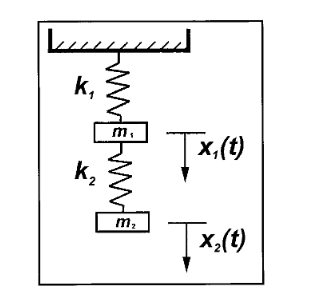
\includegraphics[width=0.3\textwidth]{E1.png}
\end{figure}

\section{No linealidad}

Si consideramos oscilaciones más grandes, el movimiento de restauracion se cuelve no lineal. Para esto tenemos que cambiar un poco las ecuaciones de modelado considerano ahora un par de coeficientes de no lienalidad como se muestra a continuacion. 

\begin{figure}[ht!]
\centering
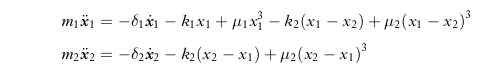
\includegraphics[width=0.3\textwidth]{E2.png}
\end{figure}

Por lo tanto proponemos ahora la sigueinte funcion al programar en jupyter lab. 

\begin{verbatim}

def vectorfield(w, t, p):
    """
    Defines the differential equations for the coupled spring-mass system.

    Arguments:
        w :  vector of the state variables:
                  w = [x1,y1,x2,y2]
        t :  time
        p :  vector of the parameters:
                  p = [m1,m2,k1,k2,L1,L2,b1,b2,u1,u2]
    """
    x1, y1, x2, y2 = w
    m1, m2, k1, k2, L1, L2, b1, b2, u1, u2 = p

    # Create f = (x1',y1',x2',y2'):
    f = [y1,
         (-b1 * y1 - k1 * (x1) + u1*(x1**3) - k2 * (x1 - x2) + u2*((x1-x2)**3)),
         y2,
         (-b2 * y2 - k2 * (x2 - x1) + u2*((x2-x1)**3))]
    return f

\end{verbatim}

\subsection{Ejemplos resueltos}

Example 3.1 Assume m1=m2=1 . Describe the motion for spring constants k1=.4 and k2=1.808, damping coefficients b1=0 and b2=0 , non linear coefficients u1=-1/6 and u2= -1/10,   with   initial   conditions (x1(0),y1(0),x2(0),y2(0))=(1,0,-1/2,0).

\begin{figure}[ht!]
\centering
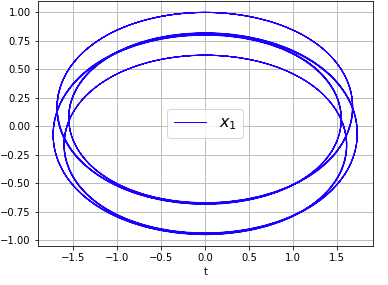
\includegraphics[width=0.3\textwidth]{311.png}
\end{figure}

\begin{figure}[ht!]
\centering
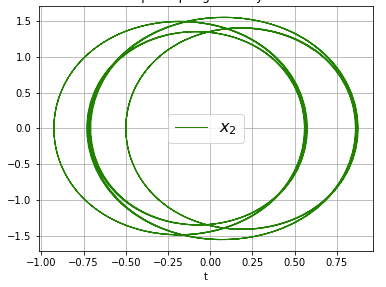
\includegraphics[width=0.3\textwidth]{312.png}
\end{figure}

\begin{figure}[ht!]
\centering
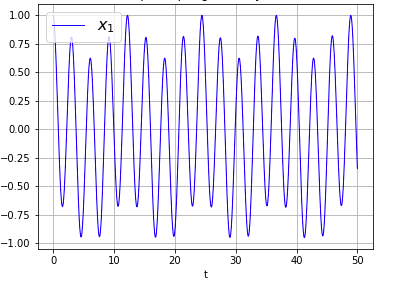
\includegraphics[width=0.3\textwidth]{313.png}
\end{figure}

\begin{figure}[ht!]
\centering
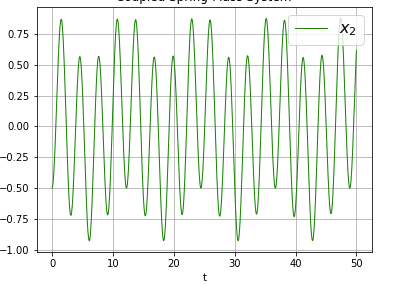
\includegraphics[width=0.3\textwidth]{314.png}
\end{figure}

\begin{figure}[ht!]
\centering
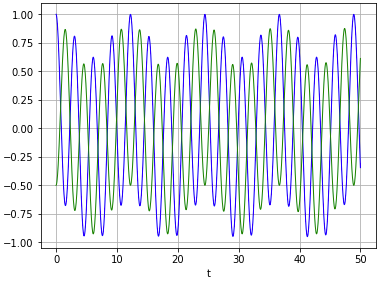
\includegraphics[width=0.3\textwidth]{315.png}
\end{figure}

\begin{figure}[ht!]
\centering
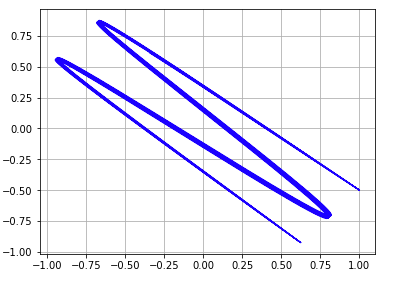
\includegraphics[width=0.3\textwidth]{316.png}
\end{figure}

\newpage


Example 3.2 Assume m1=m2=1 . Describe the motion for spring constants k1=.4 and k2=1.808, damping coefficients b1=0 and b2=0 , non linear coefficients u1=-1/6 and u2= -1/10,   with   initial   conditions (x1(0),y1(0),x2(0),y2(0))=(-.5,1/2,3.001,5.9).

\begin{figure}[ht!]
\centering
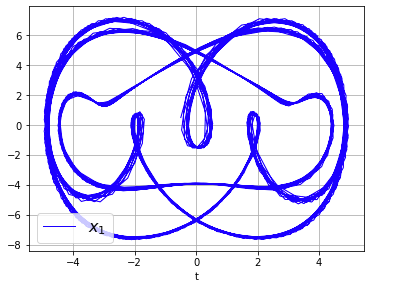
\includegraphics[width=0.3\textwidth]{321.png}
\end{figure}

\begin{figure}[ht!]
\centering
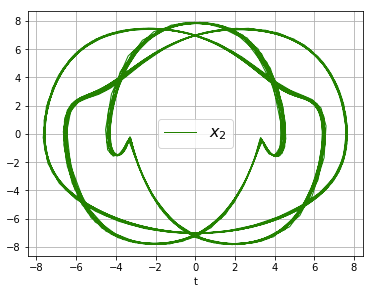
\includegraphics[width=0.3\textwidth]{322.png}
\end{figure}

\begin{figure}[ht!]
\centering
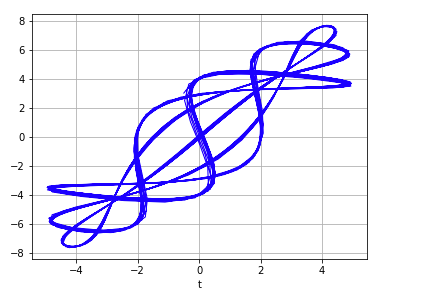
\includegraphics[width=0.3\textwidth]{323.png}
\end{figure}
\newpage


Example 3.3 Assume m1=m2=1 . Describe the motion for spring constants k1=.4 and k2=1.808, damping coefficients b1=0 and b2=0 , non linear coefficients u1=-1/6 and u2= -1/10,   with   initial   conditions (x1(0),y1(0),x2(0),y2(0))=(-.6,1/2,3.001,5.9).

\begin{figure}[ht!]
\centering
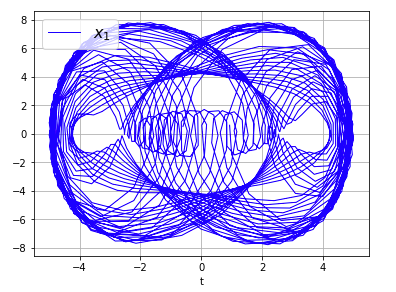
\includegraphics[width=0.3\textwidth]{331.png}
\end{figure}

\begin{figure}[ht!]
\centering
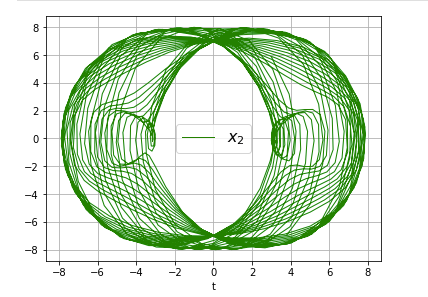
\includegraphics[width=0.3\textwidth]{332.png}
\end{figure}

\begin{figure}[ht!]
\centering
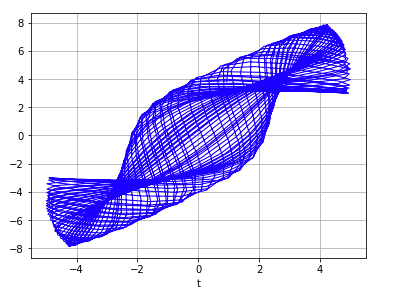
\includegraphics[width=0.3\textwidth]{333.png}
\end{figure}
\newpage

\section{Forzamiento}
Como ultimo agregado al movimieento del resorte para hacerlo aun más completo agregamos un movimiento de forazmiento, es decir que se le administra alfo de energia extra para que este no deje de oscilar. Para esto se deben considerar un par de coeficientes de forzamiento f1 y f2 al igual que un par de omegas w1 y w2 como se muestra en la ecuacion siguiente. 

\begin{figure}[ht!]
\centering
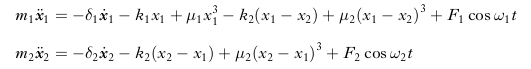
\includegraphics[width=0.3\textwidth]{E3.png}
\end{figure}

Por lo tanto al programar nuestro nuevo vector proponemos un codigo como el siguiente.

\begin{verbatim}

def vectorfield(w, t, p):
    """
    Defines the differential equations for the coupled spring-mass system.

    Arguments:
        w :  vector of the state variables:
                  w = [x1,y1,x2,y2]
        t :  time
        p :  vector of the parameters:
                  p = [m1,m2,k1,k2,L1,L2,b1,b2,u1,u2, F1, F2, w1, w2]
    """
    x1, y1, x2, y2 = w
    m1, m2, k1, k2, L1, L2, b1, b2, u1, u2, F1, F2, w1, w2 = p

    # Create f = (x1',y1',x2',y2'):
    f = [y1,
         (-b1 * y1 - k1 * (x1) + u1*(x1**3) - k2 * (x1 - x2) + u2*((x1-x2)**3) + F1*(np.cos(w1*t))),
         y2,
         (-b2 * y2 - k2 * (x2 - x1) + u2*((x2-x1)**3) + F2*(np.cos(w2*t)))]
    return f

\end{verbatim}

\subsection{Ejemplos resueltos}

Example 4.1.Assume m1=m2=1. Describe the motion for spring constants k1=2/5 and k=1, damping coefficients b1=1/10 and b2=1/5, nonlinear coefficients u1= and u2=, forcing amplitudes F1=3 and F2=5,and  forcing  frequencies w1= and w2=,  with  initial  conditions (x1(0),y1(0),x2(0),y2(0))=(-.7,0,.1,0).

\begin{figure}[ht!]
\centering
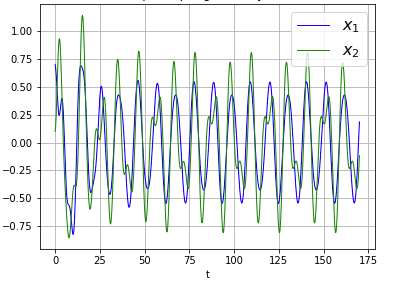
\includegraphics[width=0.3\textwidth]{411.png}
\end{figure}

\begin{figure}[ht!]
\centering
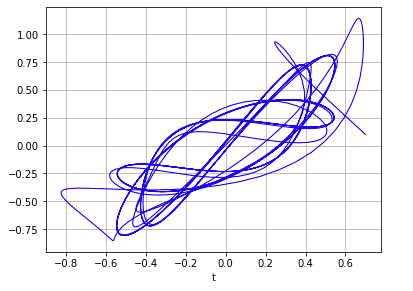
\includegraphics[width=0.3\textwidth]{412.png}
\end{figure}

\newpage

    Qué más te llama la atención de la actividad completa? ¿Que se te hizo menos interesante?
    \linebreak
    
    Se me hizo interesante lo facil que fue ir mejorando el modelo una vez acostumbrado  un poco al funcionamiento de jupyter lab. Se me hizo poco interesante graficar.
    \linebreak
    
    ¿De un sistema de masas acopladas como se trabaja en esta actividad, hubieras pensado que abre toda una nueva área de fenómenos no lineales?
    \linebreak
    En uno que se encuentra interaccionando con muchas fuerzas variantes a la vez.
    \linebreak
    
    ¿Qué propondrías para mejorar esta actividad? ¿Te ha parecido interesante este reto?
    \linebreak
    Una clase de introduccion y fue interesante.
    \linebreak
    
    ¿Quisieras estudiar mas este tipo de fenómenos no lineales?
    \linebreak
    Solo si vienen con un ejemplo muy bueno.
    
\section{Referencia}

TEMPLE H. FAY, SARAH DUNCAN GRAHAM. (2003). Coupled spring equations. 12 de abril 2017, de Taylor and Francis group Sitio 
\begin{verbatim}
web: http://math.oregonstate.edu/~gibsonn/Teaching/MTH323-010S15/Supplements/coupled_spring.pdf

\end{verbatim}


 

\end{document}